\documentclass{article}
\usepackage{amsmath}
\usepackage{amsfonts}
\usepackage{geometry}
\usepackage{booktabs}
\usepackage{tcolorbox}
\usepackage{tikz}
\usetikzlibrary{arrows.meta, patterns}

\geometry{a4paper, margin=1in}

\begin{document}

\title{Dynamics (Newton's Laws)}
\author{}
\date{}
\maketitle


\section{Newton's First Law of Motion (Law of Inertia)}

Newton's First Law states: \emph{An object at rest stays at rest, and an object in motion stays in motion with the same speed and in the same direction, unless acted upon by an unbalanced (net) force.}

\subsection{Inertia and Mass}
\textbf{Inertia} is the natural tendency of an object to resist changes in its state of motion.
\begin{itemize}
    \item Mass ($m$) is the quantitative measure of inertia. A heavier object has more inertia, meaning it is harder to start moving, stop moving, or change its direction.
    \item Inertia is \textbf{not} a force; it is a property of matter.
\end{itemize}

\subsection{Equilibrium ($\vec{F}_{\text{net}} = 0$)}
When the vector sum of all forces (the net force) acting on an object is zero, the object is in \textbf{equilibrium}.
\begin{itemize}
    \item \textbf{Static Equilibrium:} The object is at rest ($\vec{v} = 0$, $\vec{a} = 0$).
    \item \textbf{Dynamic Equilibrium:} The object is moving at a \emph{constant velocity} ($\vec{v} \neq 0$, but $\vec{a} = 0$). Constant velocity means constant speed \emph{and} straight-line direction.
\end{itemize}

\begin{figure}[h]
    \centering
    \begin{minipage}{0.45\textwidth}
        \centering
        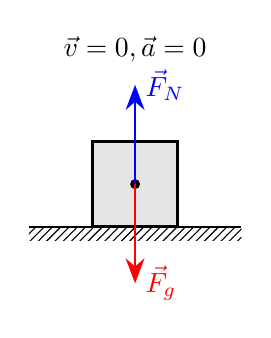
\begin{tikzpicture}[scale=0.9, line width=1pt]
            \draw[thick] (-1.5,0) -- (1.5,0);
            \fill[pattern=north east lines] (-1.5,-0.2) rectangle (1.5,0);
            \draw[fill=gray!20] (-0.6,0) rectangle (0.6,1.2);
            \fill (0,0.6) circle (2pt);
            \draw[-{Stealth[scale=1.2]}, red] (0,0.6) -- (0,-0.8) node[right] {$\vec{F}_g$};
            \draw[-{Stealth[scale=1.2]}, blue] (0,0.6) -- (0,2) node[right] {$\vec{F}_N$};
            \node at (0, 2.5) {$\vec{v} = 0, \vec{a} = 0$};
        \end{tikzpicture}
        
        \vspace{0.2cm}
        \small (a) Static Equilibrium (At rest)
    \end{minipage}%
    \hfill
    \begin{minipage}{0.45\textwidth}
        \centering
        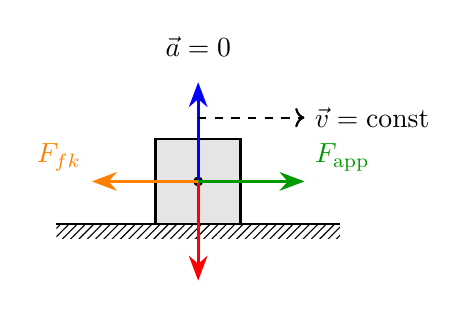
\begin{tikzpicture}[scale=0.9, line width=1pt]
            \draw[thick] (-2,0) -- (2,0);
            \fill[pattern=north east lines] (-2,-0.2) rectangle (2,0);
            \draw[fill=gray!20] (-0.6,0) rectangle (0.6,1.2);
            \fill (0,0.6) circle (2pt);
            \draw[-{Stealth[scale=1.2]}, red] (0,0.6) -- (0,-0.8);
            \draw[-{Stealth[scale=1.2]}, blue] (0,0.6) -- (0,2);
            \draw[-{Stealth[scale=1.2]}, green!60!black] (0,0.6) -- (1.5,0.6) node[above right] {$F_{\text{app}}$};
            \draw[-{Stealth[scale=1.2]}, orange] (0,0.6) -- (-1.5,0.6) node[above left] {$F_{fk}$};
            \draw[->, thick, dashed] (0, 1.5) -- (1.5, 1.5) node[right] {$\vec{v} = \text{const}$};
            \node at (0, 2.5) {$\vec{a} = 0$};
        \end{tikzpicture}
        
        \vspace{0.2cm}
        \small (b) Dynamic Equilibrium ($F_{\text{app}} = F_{fk}$)
    \end{minipage}
    \caption{Examples of objects satisfying Newton's First Law.}
\end{figure}

\newpage

\section{Newton's Second Law of Motion ($F=ma$)}

Newton's Second Law describes what happens when the net force is \emph{not} balanced. It states that the acceleration of an object is directly proportional to the net force acting upon it and inversely proportional to its mass.

\begin{equation}
\vec{F}_{\text{net}} = m\vec{a}
\end{equation}

Where:
\begin{itemize}
    \item $\vec{F}_{\text{net}}$ is the \textbf{net force} (the vector sum of all individual forces: $\sum \vec{F}$), measured in Newtons ($\text{N}$).
    \item $m$ is the \textbf{mass} of the object, measured in kilograms ($\text{kg}$).
    \item $\vec{a}$ is the \textbf{acceleration}, measured in meters per second ($\text{m/s}^2$).
\end{itemize}

\subsection{Key Concepts}
\begin{enumerate}
    \item \textbf{Vector Nature:} The acceleration $\vec{a}$ \textbf{always} points in the exact same direction as the net force $\vec{F}_{\text{net}}$.
    \item \textbf{Component Equations:} Because it's a vector equation, we usually break it down into $x$ and $y$ components when solving problems:
    \begin{equation*}
        \Sigma F_x = m a_x \quad \text{and} \quad \Sigma F_y = m a_y
    \end{equation*}
    \item \textbf{Common Mistake:} DO NOT treat $m\vec{a}$ as a force! You should never draw $m\vec{a}$ as an applied force vector on your Free-Body Diagram. It is the \emph{result} of the actual forces.
\end{enumerate}

\begin{figure}[h]
    \centering
    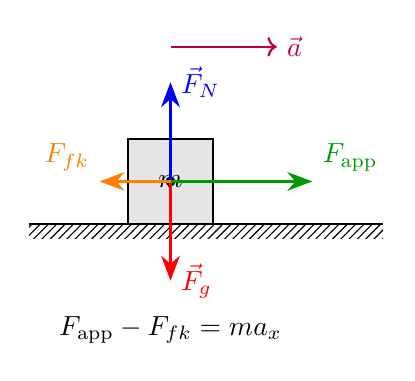
\begin{tikzpicture}[scale=0.9, line width=1pt]
        \draw[thick] (-2,0) -- (3,0);
        \fill[pattern=north east lines] (-2,-0.2) rectangle (3,0);
        
        \draw[fill=gray!20] (-0.6,0) rectangle (0.6,1.2);
        \node at (0, 0.6) {$m$};
        \fill (0,0.6) circle (2pt);
        
        \draw[-{Stealth[scale=1.2]}, red] (0,0.6) -- (0,-0.8) node[right] {$\vec{F}_g$};
        \draw[-{Stealth[scale=1.2]}, blue] (0,0.6) -- (0,2) node[right] {$\vec{F}_N$};
        \draw[-{Stealth[scale=1.2]}, green!60!black] (0,0.6) -- (2,0.6) node[above right] {$F_{\text{app}}$};
        \draw[-{Stealth[scale=1.2]}, orange] (0,0.6) -- (-1.0,0.6) node[above left] {$F_{fk}$};
        
        \draw[->, thick, purple] (0, 2.5) -- (1.5, 2.5) node[right] {$\vec{a}$};
        \node at (0, -1.5) {$F_{\text{app}} - F_{fk} = m a_x$};
    \end{tikzpicture}
    \caption{Unbalanced forces causing an object to accelerate to the right.}
\end{figure}

\newpage

\section{Newton's Third Law of Motion (Action-Reaction)}

Newton's Third Law states: \emph{Whenever one object exerts a force on a second object, the second object exerts an equal and opposite force on the first object.}

More simply: ``For every action, there is an equal and opposite reaction.''

\begin{equation}
\vec{F}_{\text{A on B}} = -\vec{F}_{\text{B on A}}
\end{equation}

\subsection{Properties of Action-Reaction Pairs}
\begin{itemize}
    \item \textbf{Same Type of Force:} If object A exerts a gravitational pull on object B, then object B exerts a gravitational pull on A.
    \item \textbf{Equal Magnitude:} Both forces are exactly the same size.
    \item \textbf{Opposite Direction:} If A pushes B to the right, B pushes A to the left.
    \item \textbf{Different Objects:} This is the most crucial point. The forces in a Third Law pair \textbf{always act on different objects}. Therefore, they \textbf{do not cancel each other out} on a single Free-Body Diagram.
\end{itemize}

\begin{figure}[h]
    \centering
    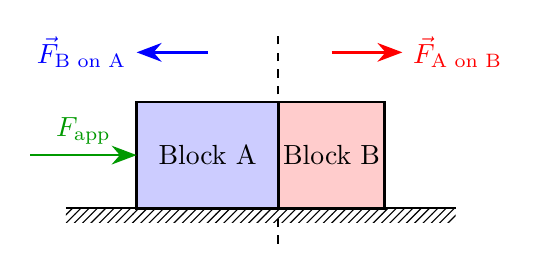
\begin{tikzpicture}[scale=0.9, line width=1pt]
        % Box A
        \draw[fill=blue!20] (-2,0) rectangle (0,1.5);
        \node at (-1, 0.75) {Block A};
        % Box B
        \draw[fill=red!20] (0,0) rectangle (1.5,1.5);
        \node at (0.75, 0.75) {Block B};
        
        % Ground
        \draw[thick] (-3,0) -- (2.5,0);
        \fill[pattern=north east lines] (-3,-0.2) rectangle (2.5,0);
        
        % Push from outside on A
        \draw[-{Stealth[scale=1.2]}, green!60!black] (-3.5, 0.75) -- (-2, 0.75) node[midway, above] {$F_{\text{app}}$};
        
        % Interacting forces
        % A on B
        \draw[-{Stealth[scale=1.2]}, red] (0.75, 2.2) -- (1.75, 2.2) node[right] {$\vec{F}_{\text{A on B}}$};
        % B on A
        \draw[-{Stealth[scale=1.2]}, blue] (-1.0, 2.2) -- (-2.0, 2.2) node[left] {$\vec{F}_{\text{B on A}}$};
        
        % Interaction boundary
        \draw[dashed, thick] (0,-0.5) -- (0,2.5);
    \end{tikzpicture}
    \caption{Block A pushes Block B to the right, so Block B pushes Block A to the left with an equal force.}
\end{figure}

\end{document}